% Background (2.75p)
\section{Background}
\label{sec:background}



\subsection{Context-aware Systems}
Context-aware systems are ones that are able to adapt their behavior according to changing circumstances without user intervention, according to Finkelstein and Savigni~\cite{finkelstein_framework_2001}.

\emph{Environment} is whatever the world provides: a surrounding in which the agent is supposed to operate. The environment comprises, for example, characteristics of the device that the agent is supposed to operate in. \emph{Context} is the reification of the environment and provides a manageable, easily computer manipulable description of the environment. Thus, a context-aware system should watch relevant environment properties and keep a runtime model that represents that information. By reasoning about that runtime model the system can change its behavior. A context can be either an activator of goals or a precondition on the applicability of certain strategies to reach a goal.

% In Finkelstein and Savigni framework, \emph{goal} is an abstract and long term objective the system should achieve. A \emph{requirement} operationalises a goal as a more concrete, short-term objective that is directly achievable through actions performed by one or more agents.
% The system should keep a causal connection between the service and the description. The system adapts by manipulating the \emph{service description}, which is the meta-level representation of the actual, real-world service. It should be a suitable formalism that allows services to be compared to requirements in order to identify runtime violations. Finally, \emph{service} provides the actual behavior as perceived by the user.

% A \emph{reflective system} is a system which incorporates structures representing (aspects of) itself. A \emph{causal connection} between a model and a element modeled exists if one of them changes, this leads to a corresponding effect upon the other~\cite{maes_concepts_1987}.

% We describe their conceptual framework for context-aware services in Figure~\ref{fig:finkelstein_framework}.
% \begin{figure}[!htb]
%   \centering
%   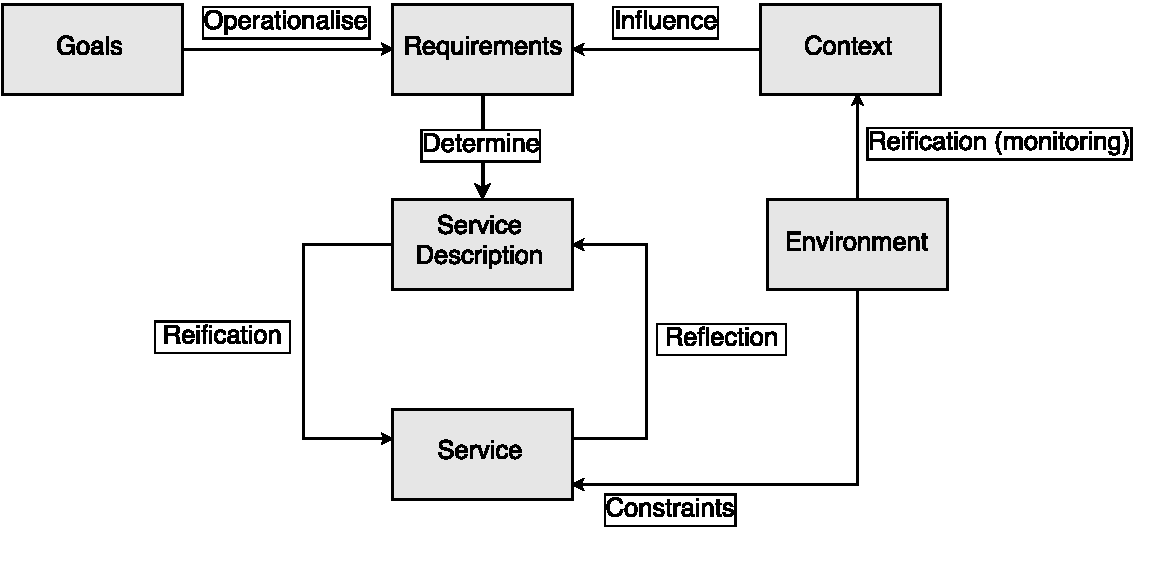
\includegraphics[width=\linewidth]{finkelstein_framework}
%   \caption{Context-aware services framework by~\cite{finkelstein_framework_2001}}
% \label{fig:finkelstein_framework}
% \end{figure}

% \textcolor{red}{This description, is still too big. Needs to be shortend.}
% Requirements reflection was also proposed~\cite{bencomo_requirements_2010} as a way of drive system adaptation.

\subsection{Goal Model and Contexts}
Goal-Oriented analysis is a requirements engineering approach that captures and documents the intentionality behind requirements. Goal-oriented Requirements Engineering (GORE) approaches have gained special attention as a technique to specify adaptable systems~\cite{morandini_goal-oriented_2009}. Goals capture the various objectives the system under consideration should achieve. In particular, Tropos\cite{bresciani_tropos:_2004} is a methodology for developing multi-agent systems that uses goal models for requirement analysis. In Tropos, requirements are represented as actors goals that are successively refined by AND/OR refinements. There are usually different ways to achieve a goal, and this is captured in goal models through multiple OR refinements.
Contextual Goal Model (CGM), proposed in~\cite{ali_goal-based_2010}, captures the relation between system goals and the changes into the environment that surround it. Context goal models extends goal models with context information. Goals and context is related by inserting context conditions on variation points of the goal model. Context Analysis is a technique that allows to derive a formula in verifiable peaces of information (facts). Facts are directed verified by the system, while a formula represents whether a context holds.

\begin{figure*}[!htb]
 \centering
 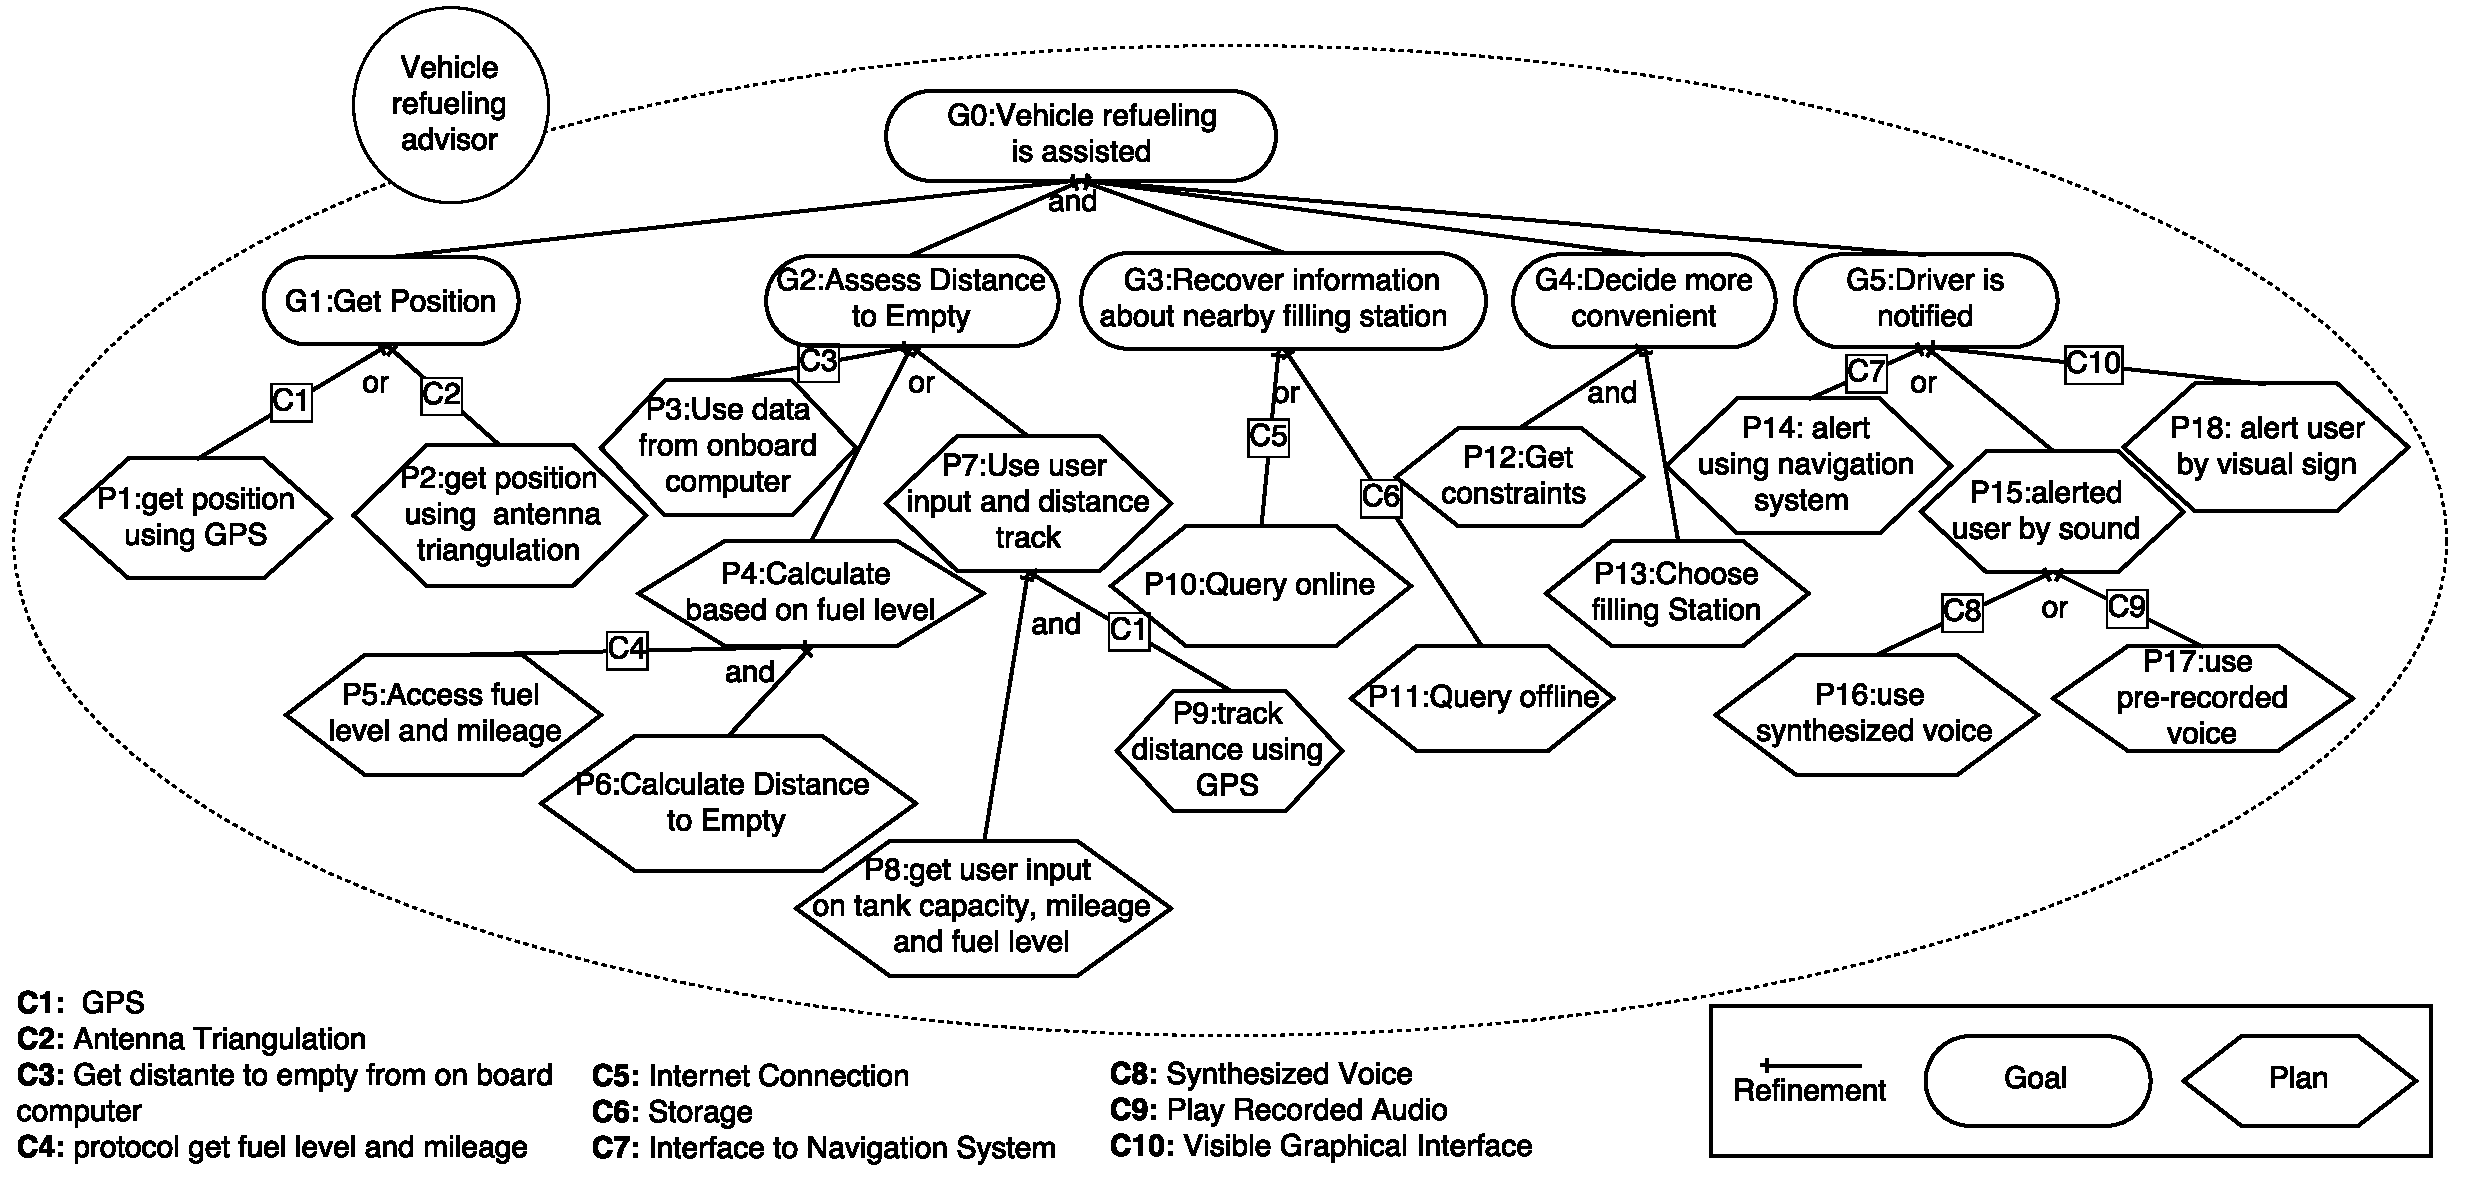
\includegraphics[width=\linewidth]{case_study/goal_model_filling_station_advisor}
 \caption{CGM of the filling station advisor}
\label{fig:goal_model_filling_station_advisor}
\end{figure*}

% \begin{figure}[!hb]
%  \centering
%  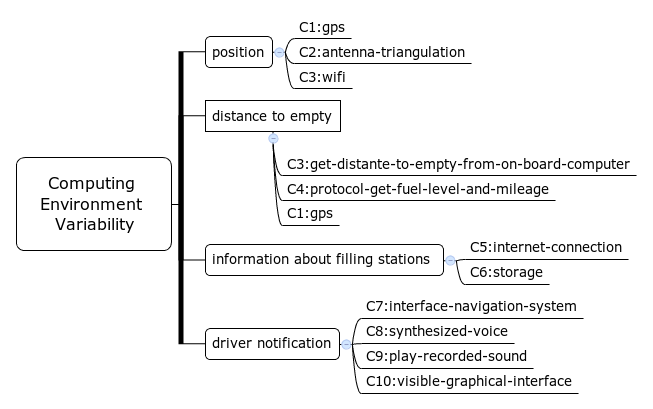
\includegraphics[width=\linewidth]{case_study/variability}
%  \caption{Variability in the Computing Environment}
% \label{fig:variability}
% \end{figure}



The CGM presented in Figure~\ref{fig:goal_model_filling_station_advisor} depicts the goals to be achieved by the Filling Station Advisor, an example application that we will use to illustrate the approach.
The main goal of the Filling Station Advisor is to give direction to a vehicle driver about nearby filling stations that can be reached conveniently. Filling station here refer to a place where the car can be refueled or recharged (gas station/petro or charge station). By convenient we mean that certain conditions for the chosen station have to be fulfilled as well as user preferences are considered. Examples of conditions are: fuel compatibility with the vehicle; whether or not the station is reachable with the amount of fuel left in the vehicle. Examples of user preferences are: low price, small deviation from an actual route, reputation of the filling station.

The root objective \emph{G0: Vehicle refueling is assisted} is AND-refined into 5 others objectives G1, G2, G3, G4 and G5. In the Goal modeling semantics it means that in order to achieve the root Goal G0, the agent should achieve the goals G1, G2, G3, G4 and G5.
\emph{G1:Get Position} has a means-end association with P1, P2 and P3. It means that the goal G1 can be achieved by executing that plans. As it is an OR-refinements, it means that G1 can be achieved by successfully executing any of the plans P1, P2 or P3. This OR-refinement introduces a variability to the system, allowing it to achieve to root goals in different ways. The contexts C1 in the association between P1 and G1 means that the Plan P1 is executable if the context C1 holds.
Context conditions on the example are of the type "required context"~\cite{ali_goal-based_2010}. These annotations means that a certain way for achieving (executing) a goal (plan) is applicable if the condition holds for the context.

%Figure~\ref{fig:variability} outlines the context space of the target computing environment. It contains variability contexts that are expected to occur in 4 subgoals of the application.

%In particular, Tropos\cite{bresciani_tropos:_2004} is a methodology for developing multi-agent systems that uses goal models for requirement analyzes. Tropos encompasses the software development phases, from Early Requirements to Implementation and Testing. Tropos use a modeling framework based on i* \cite{yu_modelling_1996} which proposes the concepts of actor, goal, plan, resource and social dependency to model both the system-to-be and its organizational operating environment \cite{bresciani_tropos:_2004} \cite{morandini_tropos_2014}. In Tropos requirements are represented as actors goals that are successively refined by AND/OR refinements. There are usually different ways to achieve a goal, and this is captured in goal models through multiple OR refinements.


%Key concepts in the Tropos metamodel are:
%
%\begin{description}%[leftmargin=6em,style=nextline]
%  \item[Actor] an entity that has strategic goals and intentionality
%
%  \item[Agent] physical manifestation of an actor.
%
%  \item[Goals] it represents actors’ strategic interests. \emph{Hard goals} are goals that have clear-cut criteria for deciding whether they are satisfied or not. \emph{Softgoals} have no clear-cut criteria and are normally used to describe preferences and quality-of-service demands.
%
%  \item[Plan] it represents, at an abstract level, a way of doing something. The execution of a plan can be a means for satisfying a goal or for \emph{satisficing} (i.e. sufficiently satisfying) a softgoal.
%
%  \item[Resource]  it represents a physical or an informational entity.
%
%  \item[Dependency] it is a relationship between two actors that specify that one actor (the \emph{depended}) have a dependency to another actor (the \emph{dependee}) to attain some goal, execute some plan or deliver a resource. The object of the dependence is the \emph{dependum}.
%
%  \item[Capability] it represents both the \emph{ability} of an actor to perform some action and the \emph{opportunity} of doing this.

  %Domain assumption

  %\item[Belief] it represents actor knowledge of the world.

%\end{description}
%
%In Tropos requirements are represented as actors goals that are successively refined by AND/OR refinements. There are usually different ways to achieve a goal, and this is captured in goal models through multiple OR refinements.

% Traditional goal models are design-time artifacts. These models are not  sufficiently detailed to reason about system execution at runtime. A design-time goal model (DGM), for example, define what plans/functions the system shall implement, but do not capture information on the status of requirements as the system is executing, nor on the history of an execution~\cite{borgida_requirements_2013}.

% Goal models are a traditionally a requirements tool, as such it must capture the space of the solution. Many works relates goal models with another aspects such as configuration, runtime execution, components

% \subsubsection{Goals}
%
% \begin{itemize}
%   \item Service
%   \item Achieve
% \end{itemize}
%

%\subsubsection{Contextual Goal Model}

%Contextual Goal Model, proposed in~\cite{ali_goal-based_2010}, captures the relation between system goals and the changes into the environment that surround it. Context goal models extends goal models with context information. Goals and context is related by inserting context conditions on variation points of the goal model. Context Analysis is a technique that allows to derive a formula in verifiable peaces of information (facts). Facts are directed verified by the system, while a formula represents whether a context holds.

% Gena: some parts of it have been mixed into Section 4.2.1
%\subsubsection{Software Components}
%Heineman defines \textit{software component} as a \say{software element that conforms to a component model and can be independently deployed and composed without modification according to a composition standard}\cite{heineman_component-based_2001}.
%
%Software components is a unit of composition. Software systems are build by composing different components.  Software components must conform to a component model by having contractually specified interfaces and explicit context dependencies only.\cite{szyperski_component_2002}.
%
%Component based software engineering (CBSE) approach consists in building systems from components as reusable units and keeping component development separate from system development\cite{crnkovic_software_2011}.
%
%A \textit{component interface} \say{defines a set of component functional properties, that is, a set of actions that’s understood by both the interface provider (the component) and user (other components, or other software that interacts with the provider)}\cite{crnkovic_software_2011}.
%A component interface has a role as a component specification and also a means for interaction between the component and its environment.
%A \textit{component model} is a set of standards for a component implementation. These standards can standardize naming, interoperability, customization, composition, evolution and deployment.\cite{heineman_component-based_2001}
%
%The \textit{component deployment} is the process that enables component integration into the system. A deployed component is registered in the system and ready to provide services\cite{crnkovic_software_2011}.
%
%\textit{Component binding} is the process that connects different components through their interfaces and interaction channels.
%
%Software architecture deals with the definition of components, their external behavior, and how they interact.\cite{kaur_component_2010}
%
%The architectural view of a software can be formalized via an architecture description language (ADL)\cite{medvidovic_classification_2000}.

%Gena: This subsection is more like a mix between related work and background. Since they are cited later in the paper with the needed parts and considering the size limitation of the paper, I commented it out.
%
%\subsubsection{From Goals to Components}
%
%Lamsweerde \cite{van_lamsweerde_system_2003} present a method to derive architecture from KAOS goal model. First an abstract draft is generated from functional goals. Secondly, the architecture is refined to meet non-functional requirements such as cohesion. The relation between software requirements and components.
%
%Pimentel et al. \cite{pimentel_deriving_2012} present a method  using i* models to produce architectural models in Acme~\cite{}. It focuses in he development of adaptive systems. First, it transforms a i* model into a modular i* model by means of horizontal transformation. Secondly, it creates an architecture model from the i* modularized model by means of vertical transformation. Architectural design models is made easier by the presence of actor and dependency concepts.
%
%Yu et al. proposed an approach for keep the variability that exists in the goal model into the architecture.
%It presents a method for creating a component-connector view from a goal model\cite{yu_goals_2008}.
%A preliminary component-connector view is generated from a goal model by creating an interface type for each goal. The interface name is directly derived from the goal name. Goals refinements result in implementation of components. If a goal is And-decomposed, the component has as many \emph{requires} interfaces as subgoals.
%
%\begin{lstlisting}
%Component G {
%  provides IG;
%  requires IG1, IG2;
%}
%\end{lstlisting}
%
%If the goal is OR-decomposed, the interface type of subgoals are the interface type of the parent goal.
%%It's the most important patterns as it allow variability at architecture.
%
%\begin{lstlisting}
%Component G1 {
%  provides IG;
%}
%
%Component G2 {
%  provides IG;
%}
%\end{lstlisting}
%
%A component equivalent to the parent goal is generated with a switch. Input and outputs are added to the interface. Related lower level components can be merged by parametrization.

\subsection{Software Deployment}

Software deployment refers to all the activities that make a software system available for use\cite{carzaniga_characterization_1998}. These activities results
in the creation and distribution of artifacts,  from the development environment to the target runtime environment. Artifacts are files that package software components and assets.

%In embedded platforms the deployment can consist in burn software into a chip. In consumer personal or business domain, for a desktop platform, the deployment can consist in a install process with collaboration between a person and a script that automate some steps. In a enterprise domain, for a web platform in can consist in coping and editing some files in a couple of machines. In many of this scenarios software will be periodically updated, frequently being unavailable in the process.
% The complexity of software deployment can also vary according to the network size and complexity, its heterogeinety, and the knowledge about the deployment computing environment at design-time. In a highly heterogeneous environment, deployment can be specially complex.


\begin{figure}[!htb]
  \centering
  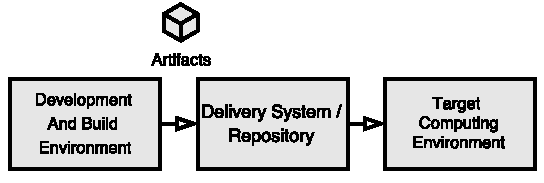
\includegraphics[width=.7\linewidth]{deployment_extended_process}
  \caption{Artifacts Deployment}
  \label{fig:deployment_extended_process}
\end{figure}

Figure~\ref{fig:deployment_extended_process} depicts the major environments in software deployment.  In the development and build environment, artifacts are built, packaged and implemented using version control system and development tools. Built artifacts are moved into a delivery system where they can be accessed, e.g., from a web site, an app store or simply a package repository. From a delivery system artifacts can be moved to a target computing environment. Once moved to the target computing environment, configuration activities can be realized.

In the software industry, a \emph{continuous integration} environment applies automation in building and getting components ready to delivery. In such an environment, if a developer pushes changes to a code repository at design-time, components are automatically built and published to the delivery system. The build process commonly involves fetching build dependencies, source code compilation, automated quality control (e.g. integration tests and static analysis) and packaging. If target quality policies are met, the artifacts can be published to a delivery system. From the delivery system, the artifacts can be copied to the target environment.
%dependency manager

%\textcolor{red}{doesn't seem to me you need this. Remove it, unless you implement such tool!
%Fundamental to continuous integration environments are \emph{Package Management Systems} (PMS) tools, which simplify the process of managing software dependencies~\cite{spinellis_package_2012}. The use of PMS tools ensure that development team members are working with same dependencies that are used in the build environment.
%
%%build manager
%\emph{Continuous delivery} extends the continuous integration environment, moving components from the delivery system to a target computing environment with none or minimum human intervention. In modern enterprise environments the deployment activity has seen significant changes with popularization of use of virtual machines and cloud computing.
%%package managers, virtual machine, middleware support
%
%Devops\cite{bang_grounded_2013} is a movement in software industry that advocates that all configuration steps needed to configure the computing environment should be written as code (\emph{infrastructure as code}), and follow best practices of software development. That movement favor the documentation, reproducibility, automation and scalability.
%%Tools such as Puppet and Chef are used by devopers to manage infrastructure.
%Devops allow for management of scalable computing environments. It can offer significant advantage for enterprise environment in relation to manual approaches in which system administrators configure the system by manually following configuration steps.
%
%Current continuous integration/delivery and devops practices are not sufficient for highly dynamic and heterogeneous computing environments; they requires that highly specialized system administrators to analyze the environment and create build pipelines and create environment configuration descriptors.}

%Most approaches for automatic software deployment use tools and languages separated from the software itself. Such approaches manage different kinds of deployment resources, such as services, files, and configuration within a file. They provide a way where deployment specialist provide boilerplate execution instructions in order to put software under execution. Such approaches are successful in deployment of large scale infrastructure such as Netflix video stream network. However, they are not suitable for the emerging dynamic heterogeneous environments in the context of self-adaptive systems.
